%% ACM sigconf draft for MARVIN
%\documentclass[sigconf]{acmart}
\documentclass[manuscript,screen]{acmart} % single col for review

%% TODO: replace with actual conference information
\setcopyright{acmlicensed}
\copyrightyear{2025}
\acmYear{2026}
\acmDOI{XXXXXXX.XXXXXXX} % TODO
\acmConference[TEI SDC '26]{TEI Student Design Challenge}{March, 2026}{Chicago, Illinois}
\acmISBN{978-1-4503-XXXX-X/2026/06} % TODO

\AtBeginDocument{\providecommand\BibTeX{{Bib\TeX}}}

\begin{document}

\title{MARVIN: Remote Teleoperation of a Dual-Arm Upper-Body Avatar Robot}
\subtitle{Real-time human motion mirroring with client-side ML and ROS2}

%% Authors
\author{Jaeho Cho}
\authornote{Both authors contributed equally to this research.}
\email{jaeho.cho@cooper.edu}
\affiliation{%
  \institution{The Cooper Union for the Advancement of Science and Art}
  \city{New York}
  \state{New York}
  \country{USA}
}
\author{Sophia Klymchuk}
\authornotemark[1]
\email{sophia.klymchuk@cooper.edu}
\affiliation{%
  \institution{The Cooper Union for the Advancement of Science and Art}
  \city{New York}
  \state{New York}
  \country{USA}
}

\renewcommand{\shortauthors}{Last}

\begin{abstract}
MARVIN is a dual-arm teleoperational robot that mirrors a human 
operator's upper-body motion in real time using just a standard webcam. 
Client-side MediaPipe models extract 3D pose and hand landmarks, which are 
transmitted via websocket to a ROS2-MoveIt servoing stack that commands two 
OpenManipulator-X arms. We detail perception-to-actuation mappings, including 
geometric formulations for shoulder flexion, shoulder abduction/adduction, and 
elbow flexion, and describe a web interface that enables intuitive interaction. 
We report latency, accuracy, and user study results from local and remote 
operation, discuss safety and failure modes, and outline pathways toward 
full-body telepresence. % edit last line to match whatever
\end{abstract}

%%
%% The code below is generated by the tool at http://dl.acm.org/ccs.cfm.
%%
\begin{CCSXML}
<ccs2012>
   <concept>
       <concept_id>10010583</concept_id>
       <concept_desc>Hardware</concept_desc>
       <concept_significance>500</concept_significance>
       </concept>
 </ccs2012>
\end{CCSXML}

\ccsdesc[500]{Hardware}

\keywords{teleoperation, human-robot interaction, ROS2, MoveIt, MediaPipe}

\received{NA} % TODO
\received[revised]{NA} % TODO
\received[accepted]{NA} % TODO

\maketitle

\section{Introduction}
MARVIN is a teleoperational robot that mirrors the upper-body movements of a 
human operator in real time. Operation works via a local webcam or a remote 
connection, where a web application captures the user's webcam 
stream for pose landmarking, enabling MARVIN to act as a physical avatar across 
any distance.

MARVIN explores the theme of the 2026 SDC theme of Sensory Rituals through the 
design of a remotely-operated humanoid robot that reintroduces physicality 
into digital communication. 
Contemporarily, much of interpersonal digital interaction occurs via screen-based 
interfaces that flatten embodied and sensory engagement. Via MARVIN, we seek to
restore a sense of physical presence to virtual meetings by allowing its users to
inhabit a robot equipped with two controllable arms.

By remotely manipulating the robot via one's own mirrored actions, tangible social 
connection can be had at-distance, enabling the operator to perform actions, express
intentions, and interact with physical environments shared by the receiver.

Furthermore, MARVIN is an accessible platform, as it requires only a standard 
webcam and Internet interface, which extends this ritual to anyone irrespective 
of distance, with only minimal technological barriers. This inclusivity broadens 
the system's use as a tool for fostering shared sensory experiences in remote or 
hybrid environments. Via its integration of presence, interaction, and accessibility, 
MARVIN allows tangible rituals to emerge out of traditional confinement and into 
a process of technological mediation that reconnects individuals to the physical world
and to one another.

% \section{Related Work}
% TODO: Add literature comparison and related teleoperation frameworks.

\section{Hardware}
MARVIN uses components from the ROBOTIS OpenManipulator-X platform. Each arm has 
5 DOF and is powered by Dynamixel XM430-W350 servos. We utilize two arms attached 
to an aluminum-beam torso and powered via a Dynamixel U2D2 power hub.

\section{Software}
MARVIN runs on the Humble distribution of ROS2. High-level motion is handled by 
MoveIt, which translates user commands into low-level commands sent to Dynamixel 
controllers. A custom URDF/Xacro model encodes simultaneous kinematics, 
inertial, and control interfaces for both arms.

\subsection{Pose Detection}
OpenCV interfaces a MediaPipe-based pose detector to extract 
normalized 3D joint landmarks from a webcam stream \cite{noauthor_mediapipe_nodate}. 
We use shoulder (11,12), elbow (13,14), wrist (15,16), and hip 
(23,24) landmarks to compute joint angles that are then 
mapped to MARVIN's kinematic model. Figure \ref{fig:pose-landmarks}
displays the landmark labelling scheme.

\begin{figure}[htbp]
  \centering
  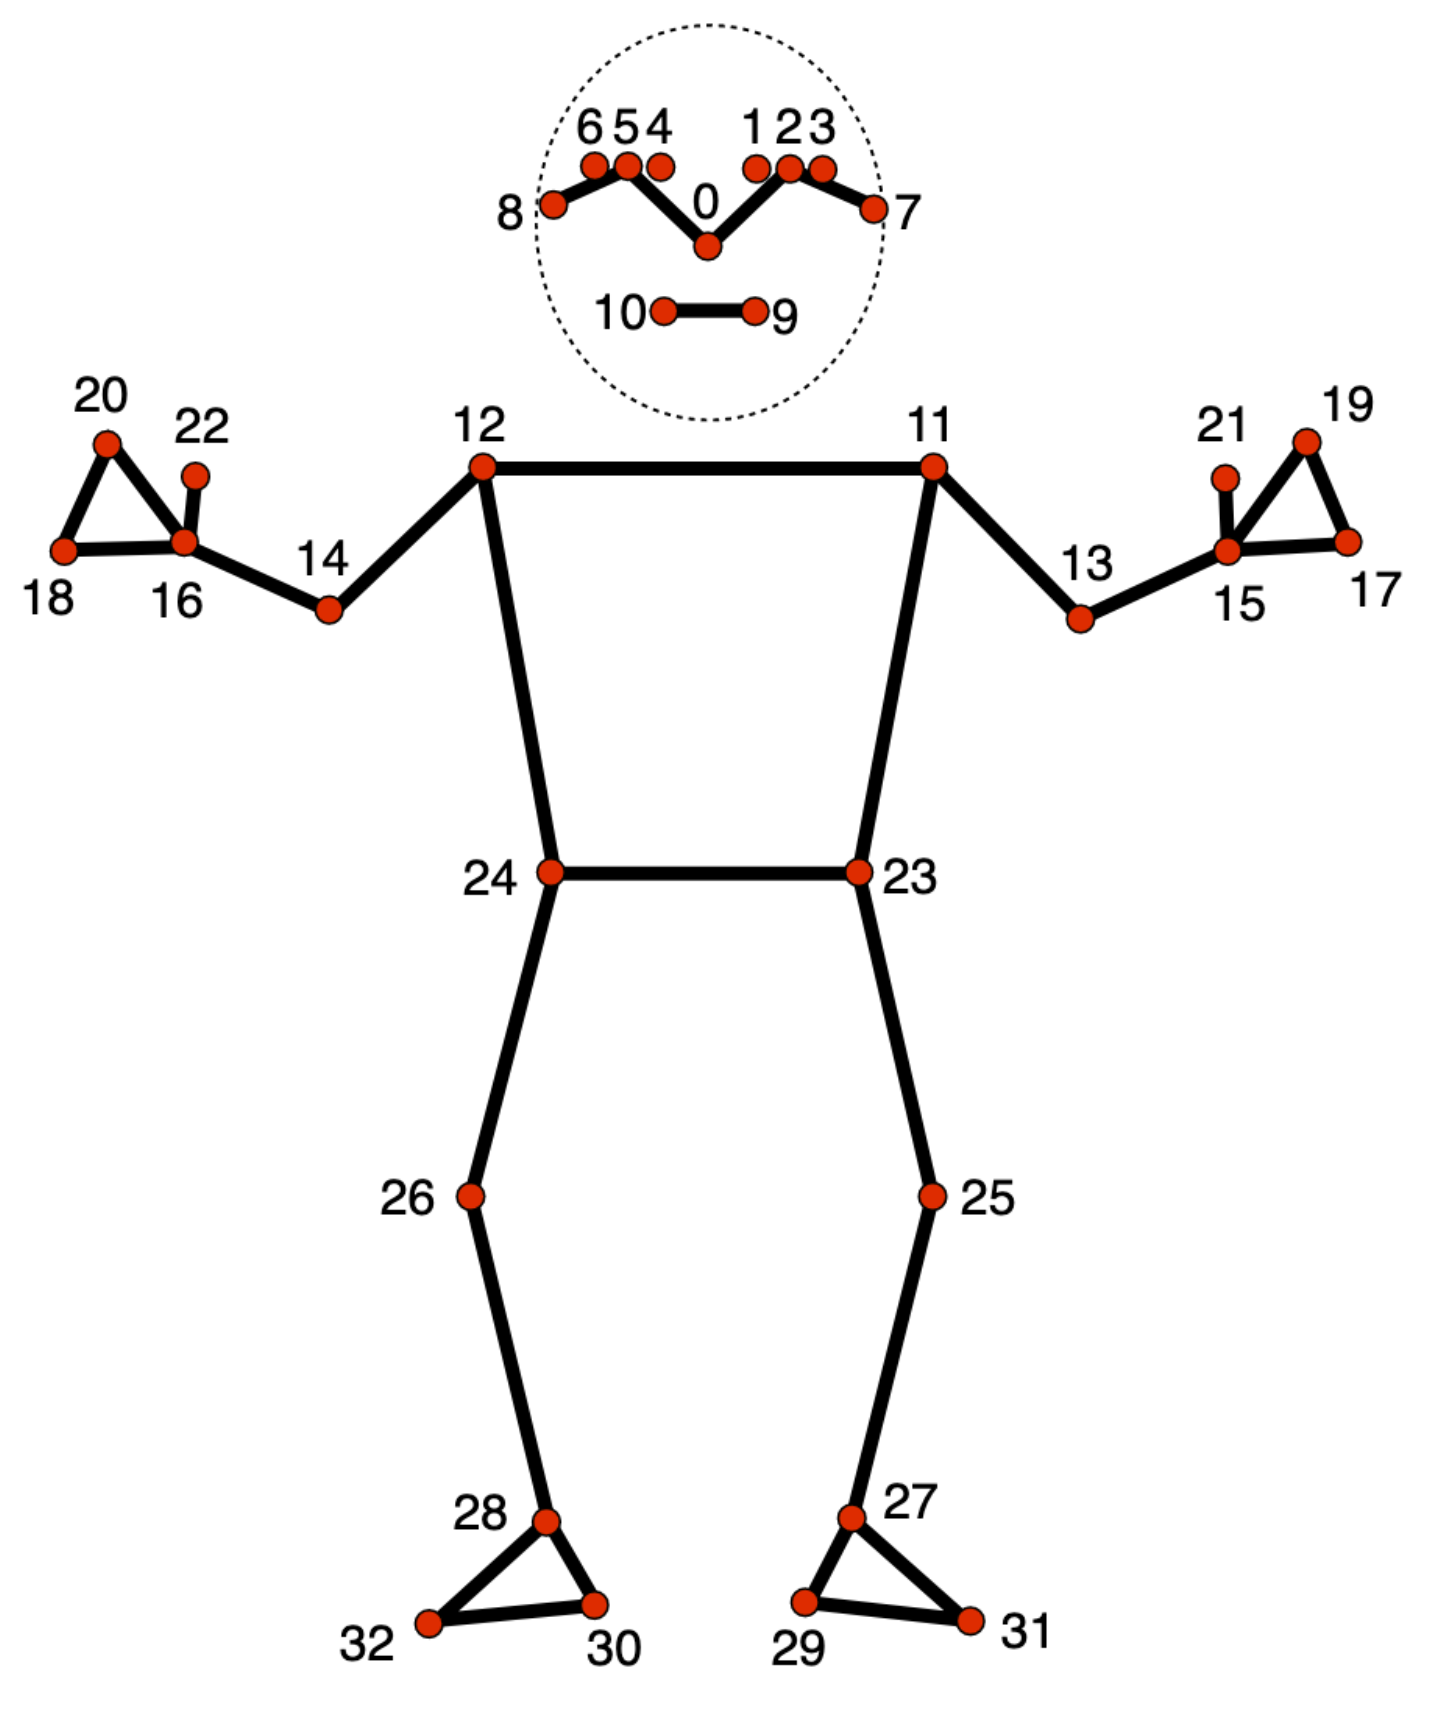
\includegraphics[width=0.5\linewidth]{assets/pose-landmarks.png}
  \caption{MediaPipe Pose Landmarks. The pose landmarker model tracks 33 body landmark locations, representing the approximate location of the labeled body parts.}
  \Description{A diagram of a human figure with 33 labeled landmarks, including shoulders, elbows, wrists, hips, knees, and ankles.}
  \label{fig:pose-landmarks}
\end{figure}

\subsubsection{Shoulder Flexion}
Let $S$ (shoulder), $E$ (elbow), $H$ (same-side hip), $H_{opp}$ (opposite hip).
\begin{displaymath}
  \mathbf{u}=E-S,\quad \mathbf{v}=H-S,\quad \mathbf{h}=H_{opp}-H,\quad \hat{\mathbf{n}}=\frac{\mathbf{h}}{\lVert\mathbf{h}\rVert}
\end{displaymath}
Project onto the midline plane orthogonal to $\hat{\mathbf{n}}$:
$
\mathbf{u}_\pi=\mathbf{u}-(\mathbf{u}\cdot\hat{\mathbf{n}})\,\hat{\mathbf{n}},\quad
\mathbf{v}_\pi=\mathbf{v}-(\mathbf{v}\cdot\hat{\mathbf{n}})\,\hat{\mathbf{n}}. \\
$
Flexion:
\begin{equation}
\alpha=\arccos \!\left( \frac{\mathbf{u}_\pi \cdot \mathbf{v}_\pi}{\lVert\mathbf{u}_\pi\rVert\, \lVert\mathbf{v}_\pi\rVert} \right)\,.
\end{equation}
Map $\alpha$ to shoulder flexion/extension joint ($J_1$).

\subsubsection{Shoulder Adduction/Abduction}
Let $\mathbf{u}$, $\hat{\mathbf{n}}$ be as above. Project $\mathbf{u}$:
$
\mathbf{u}_\pi=\mathbf{u}-(\mathbf{u}\cdot\hat{\mathbf{n}})\,\hat{\mathbf{n}}.\\
$
Adduction magnitude:
\begin{equation}
\beta=\arccos \!\left( \frac{\mathbf{u}\cdot\mathbf{u}_\pi}{\lVert\mathbf{u}\rVert\, \lVert\mathbf{u}_\pi\rVert} \right)\,.
\end{equation}
Signed ab/adduction can be obtained from $\operatorname{sign}\big((\mathbf{u}\times\mathbf{u}_\pi)\cdot\hat{\mathbf{n}}\big)$. Map to $J_2$.

\subsubsection{Elbow Flexion}
Let $\mathbf{u}$ be as above and forearm $\mathbf{f}=E-W$. Then
\begin{equation}
\theta=\arccos \!\left( \frac{\mathbf{u}\cdot\mathbf{f}}{\lVert\mathbf{u}\rVert\, \lVert\mathbf{f}\rVert} \right)\,.
\end{equation}
Map $\theta$ to elbow joint $J_3$.

\subsubsection{Hand Open/Close}
Using the Hand Landmarker (labels shown in Figure \ref{fig:hand-landmarks}), 
define a reference length from wrist (0) to middle-finger MCP (9). 
We mark a hand as open if fewer than three fingertips among indices 
\{4,8,12,16,20\} lie closer to the wrist than the reference. We then 
publish binary open/closed messages to drive the gripper.

\begin{figure}[htbp]
  \centering
  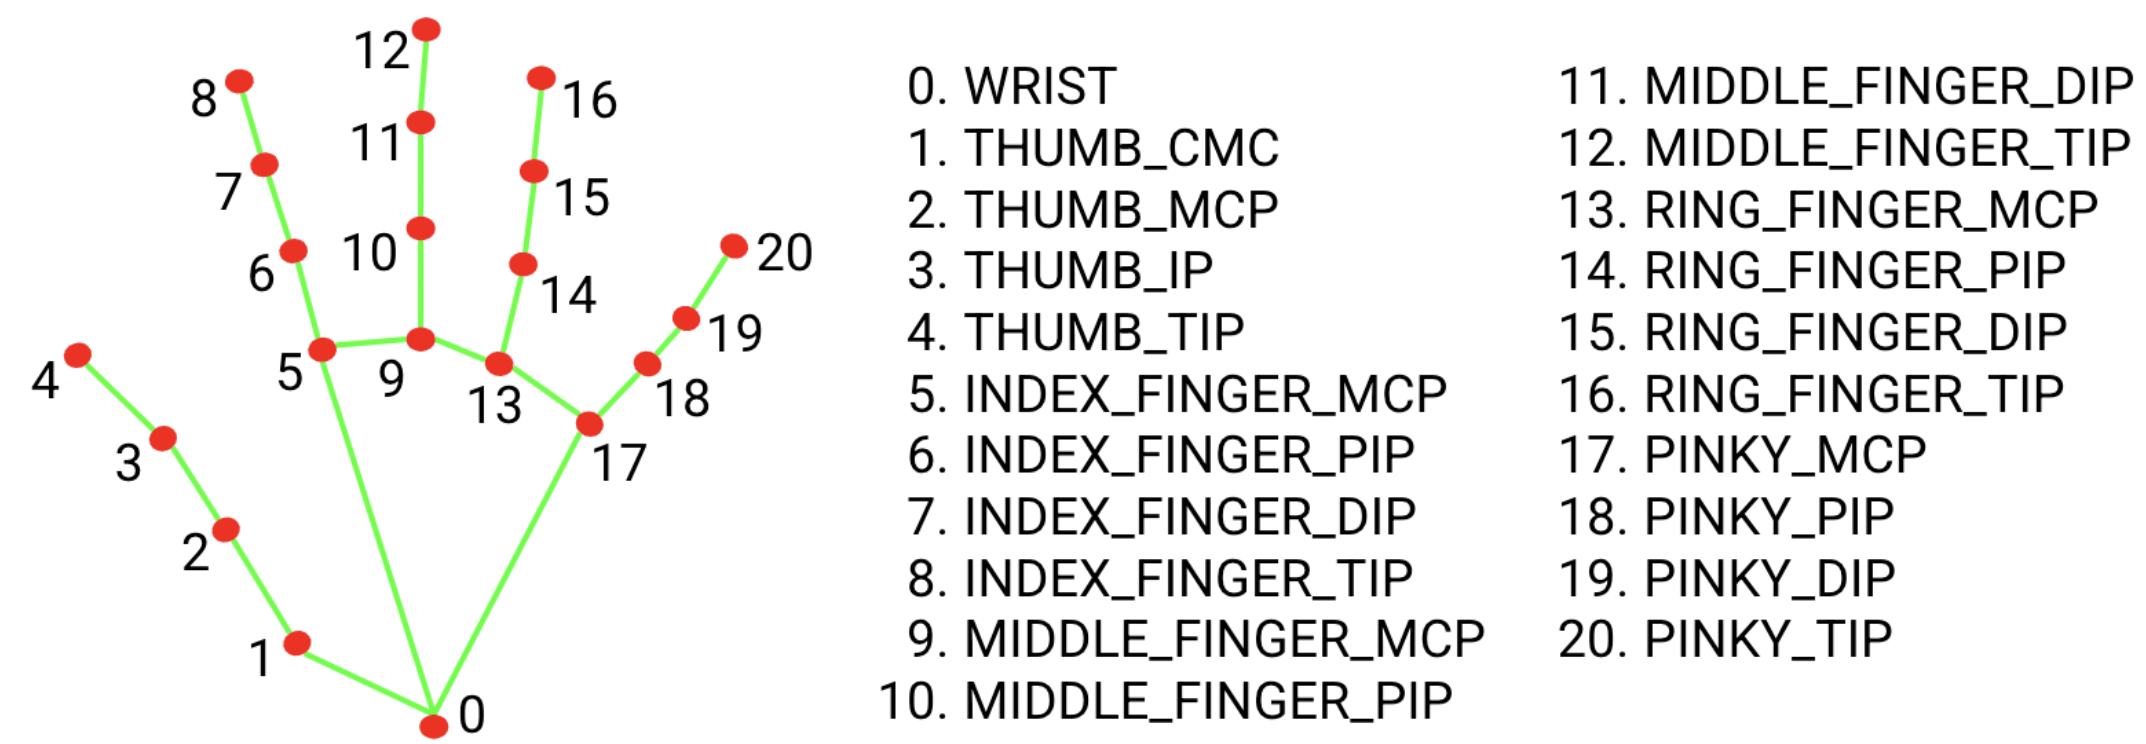
\includegraphics[width=0.5\linewidth]{assets/hand-landmarks.png}
  \caption{MediaPipe Hand Landmarks. The hand landmark model bundle detects the keypoint localization of 21 hand-knuckle coordinates within the detected hand regions.}
  \Description{A diagram of a hand with 21 labeled landmarks, including wrist, palm, and finger joints.}
  \label{fig:hand-landmarks}
\end{figure}

\subsection{Control}
We use MoveIt real-time servoing with two independent kinematic chains, one per arm. 
Each chain is associated with a servoing node that subscribes to desired joint 
velocities. These velocities are computed from the error between detected 
target joint angles and current joint states from the \texttt{/joint\_states} 
topic, before being scaled by gains and sent as \texttt{JointJog} commands.

\section{Website}
The MediaPipe Pose \& Hands — ROSBridge webpage functions as the browser-based 
front end of MARVIN’s remote teleoperation system. It captures the user’s webcam 
stream, performs on-device pose and hand landmark inference, and transmits the 
resulting kinematic data to the ROS2 backend in real time. The interface also 
embeds a live video stream of the robot, allowing visual feedback during operation. 
Implemented entirely in client-side JavaScript using the MediaPipe Tasks API, 
the system requires no native installation or external dependencies. 
A compact control panel enables users to start or stop the camera, select inference 
model complexity, and toggle streaming to the ROSBridge server, which exposes 
\texttt{pose\_landmarks} and \texttt{hand\_landmarks} topics for downstream 
motion control.

Detected landmarks are overlaid directly on the live video feed, and the interface 
reports both frame rate and end-to-end latency to the ROSBridge server, enabling 
quantifiable performance evaluation under varying network conditions. Hand 
openness is computed geometrically from landmark distances, and both hand-state 
and pose data are serialized into ROS-compatible JSON messages. This design 
supports seamless integration with MARVIN’s MoveIt servoing pipeline, where 
landmark-derived joint angles are mapped to actuator commands for real-time 
mirroring of human motion.

\begin{figure}[htbp]
  \centering
  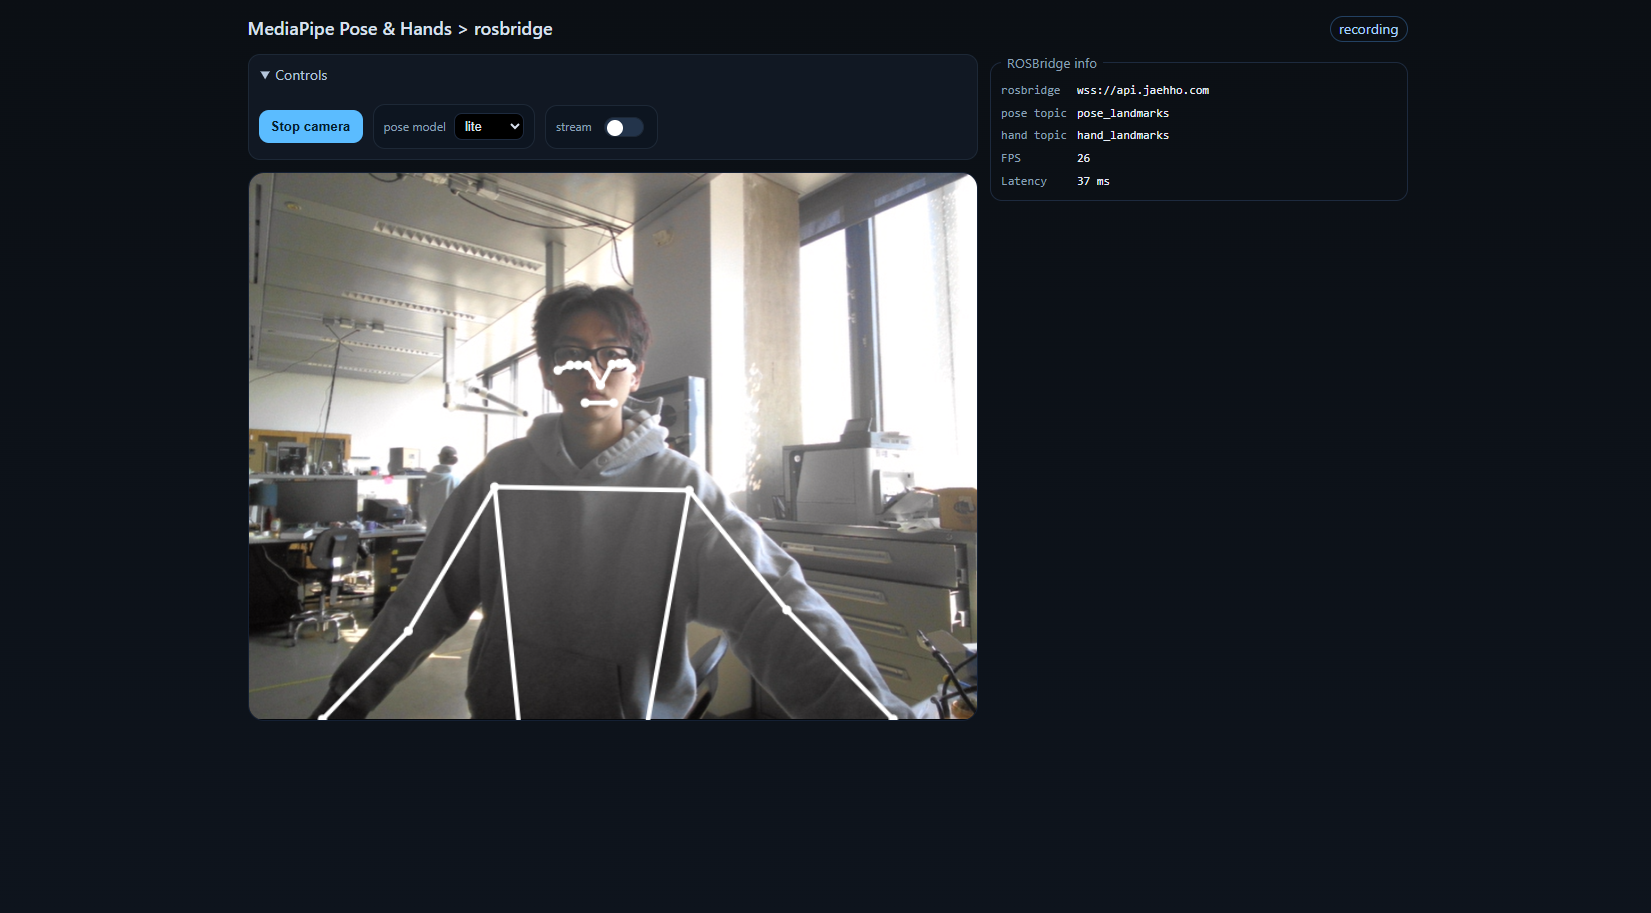
\includegraphics[width=\linewidth]{assets/web-ui}
  \caption{Browser UI for teleoperation. TODO: elaborate.} % TODO
  \Description{A screenshot of the web interface showing video feed, control buttons, and status indicators.}
  \label{fig:ui}
\end{figure}

\begin{figure}[htbp]
  \centering
  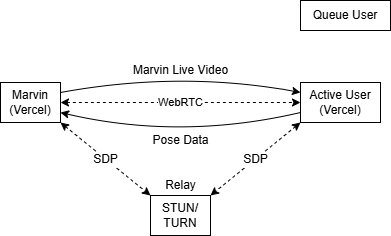
\includegraphics[width=\linewidth]{assets/system-diagram}
  \caption{ROS rqt graph overview. TODO: elaborate.} % TODO
  \Description{TODO} % TODO
  \label{fig:system}
\end{figure}

\begin{figure}[htbp]
  \centering
  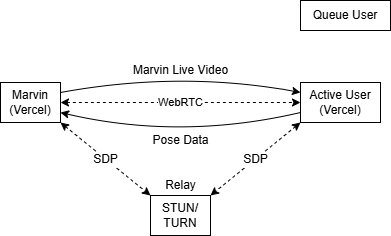
\includegraphics[width=\linewidth]{assets/system-diagram.png}
  \caption{Communication pipeline and timing. TODO: elaborate.} % TODO
  \Description{TODO} % TODO
  \label{fig:pipeline}
\end{figure}

\begin{figure}[htbp]
  \centering
  \includegraphics[width=0.5\linewidth]{assets/marvin}
  \caption{MARVIN hardware. Front and oblique views of the dual-arm upper-body platform with aluminum-beam torso, two 5-DOF OpenManipulator-X arms, and parallel grippers. Insets show Dynamixel XM430-W350 servos, U2D2 hub, and mounting.}
  \Description{Photographs of MARVIN from multiple angles highlighting mechanical structure, actuators, and end-effectors.}
  \label{fig:photos}
\end{figure}

\section{Operation and User Study}
MARVIN was tested in local operation during the Cooper Union End of 
Year Show of May 2025. The robot mirrored onlooker movements in real time, 
and we received qualitative feedback requesting the addition of hand 
gestures for a more natural feeling. This informed subsequent implementation 
of the hand landmark module and gripper control. 

We additionally tested remote operation of MARVIN with peer volunteers from the Cooper Union
community, achieving low latency? blah blah. % JAEHO

\subsection{Latency}\label{sec:latency}
We define end-to-end latency as camera exposure to actuator motion onset. 
We report median and 95th percentile latencies for both conditions, 
along with landmark inference time and ROSBridge transmission time.

\begin{table}[htbp]
  \caption{Performance summary (illustrative; replace with measured data).}
  \label{tab:perf}
  \begin{tabular}{lrr}
    \toprule
    Metric & Local & Remote \\
    \midrule
    End-to-end latency (ms) &  \textit{TODO} & \textit{TODO} \\
    Pose inference (ms/frame) & \textit{TODO} & \textit{TODO} \\
    FPS (avg) & \textit{TODO} & \textit{TODO} \\
    Task success rate (\%) & \textit{TODO} & \textit{TODO} \\
    NASA-TLX (0--100) & \textit{TODO} & \textit{TODO} \\
    \bottomrule
  \end{tabular}
\end{table}

\section{Safety and Limits}
We enforce velocity, position, and torque limits at the controller. 
We apply workspace clamping and filtering of pose outliers using 
temporal smoothing. 
Failure modes include landmark jitter, partial occlusion, and network loss. 
A dead-man switch disables actuation when no fresh landmarks arrive 
within a timeout.

% \section{Results}
% % Summarize quantitative and qualitative findings after you add data
% We observe that local operation achieves lower latency and higher success rates than remote. Participants report higher presence locally. Grasp success correlates with hand-state classification accuracy.

\section{Discussion}
MARVIN demonstrates that fully client-side inference is viable for dual-arm mirroring. Remaining gaps include wrist pronation supination estimation, depth ambiguity in monocular input, and gripper force control. Future work includes fusing depth, adding self-calibration, and extending to mobile bases for whole-body telepresence.

\section{Ethical and Societal Impact}
Telepresence expands access but raises safety and privacy concerns. We log minimal data, anonymize telemetry where possible, and provide hard e-stop. Future deployments must consider operator authentication and bystander consent in public spaces.

\section{Conclusion}
We provided a browser-first teleoperation system that minimizes setup while retaining precise, low-latency control of a dual-arm avatar robot. We plan to release code and evaluation datasets.

\begin{acks}
We thank the Cooper Union community for volunteering and supporting facilities.
\end{acks}

\bibliographystyle{ACM-Reference-Format}
\bibliography{references} % TODO: verify references.bib completeness

\appendix
\section{Angle Mapping and Calibration}
We recommend a short calibration where the operator performs canonical poses to establish shoulder plane and joint-neutral offsets. Offsets are subtracted from observed angles before mapping to robot joints.

\section{Implementation Details}
Browser stack: TypeScript, WebAssembly MediaPipe Tasks. ROSBridge schema and message formats are in the repository. Build and launch instructions for both simulation (Gazebo/Ignition) and hardware are provided.

\end{document}
